\documentclass{beamer}
\usepackage{lmodern}
\usepackage{siunitx}
\usepackage[version=3]{mhchem}
\graphicspath{{material/}}

\newcolumntype{C}{>{\centering\arraybackslash} m{0.1cm} }  %# New column type
\newcolumntype{V}{>{\centering\arraybackslash} m{0.45\linewidth} }

\title{Energy Reconstruction at High Energies}
%\subtitle{Test with KLG4}
\author[Michinari]{Michinari Sakai}
%\date

\begin{document}

\frame{\titlepage}

\begin{frame}
	\frametitle{KLG4 e-type lepton energy reconstruction using KAT}
	\framesubtitle{vertex $R < \SI{600}{cm}$, no residual nucleus}
	\begin{columns}[T]
		\column{0.3\textwidth}
		\ce{e^{-}}
		\includegraphics[width=1.0\textwidth]{analyzed_mtq_flatSpectrum_e-_outerBufferFillAll_reconVSTrueEnergy_maxR600cm.pdf}
		\column{0.3\textwidth}
		\ce{\nu_{e} + ^{1}H -> e^{-} + ?}
		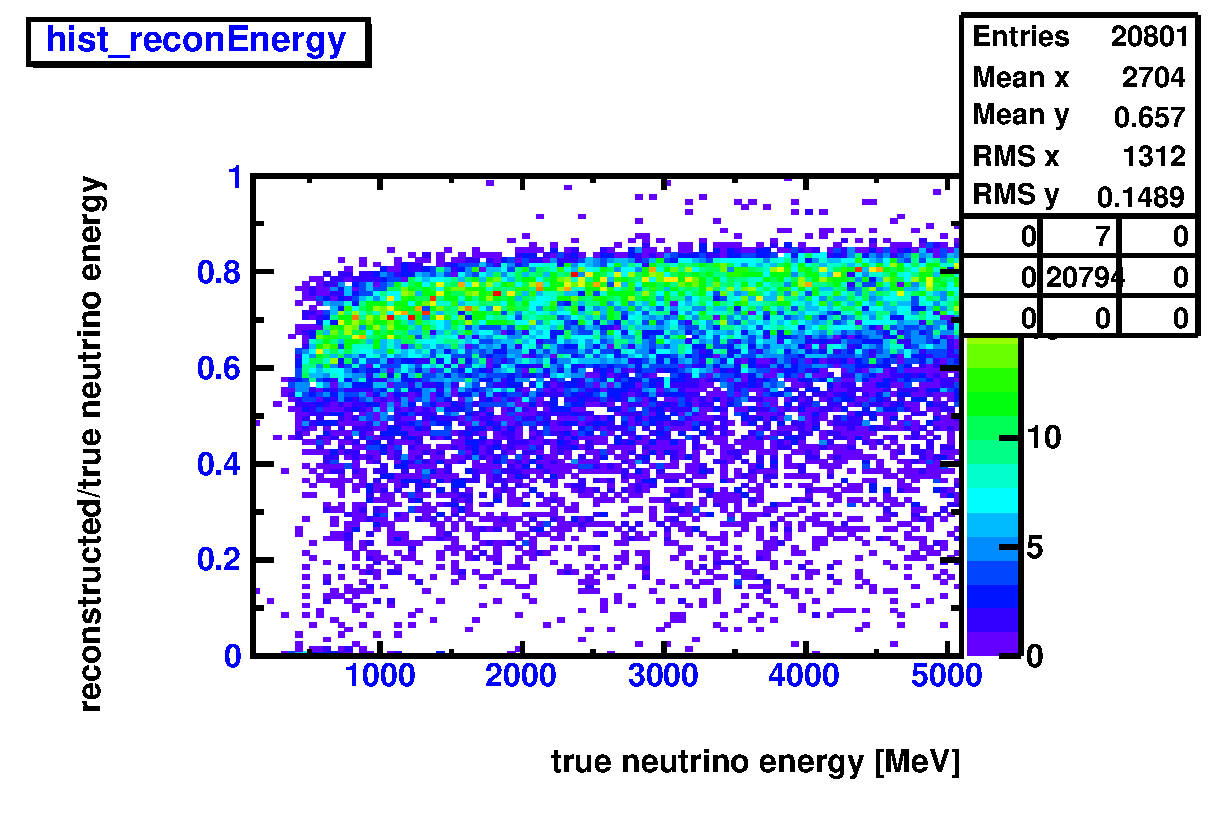
\includegraphics[width=1.0\textwidth]{nue_H1_reconVSTrueNuEnergy_onlyCC_maxR600cm.eps}
		\column{0.3\textwidth}
		\ce{\nu_{e} + ^{12}C -> e^{-} + ?}
		\includegraphics[width=1.0\textwidth]{nue_C12_reconVSTrueNuEnergy_onlyCC_maxR600cm.eps}
	\end{columns}
\end{frame}

\begin{frame}
	\frametitle{KLG4 $\mu$-type lepton energy reconstruction using KAT}
	\framesubtitle{vertex $R < \SI{600}{cm}$, no residual nucleus}
	\begin{columns}[T]
		\column{0.3\textwidth}
		\ce{\mu^{-}}
		\includegraphics[width=1.0\textwidth]{analyzed_mtq_flatSpectrum_mu-_outerBufferFillAll_reconVSTrueEnergy_maxR600cm.pdf}
		\column{0.3\textwidth}
		\ce{\nu_{\mu} + ^{1}H -> \mu^{-} + ?}
		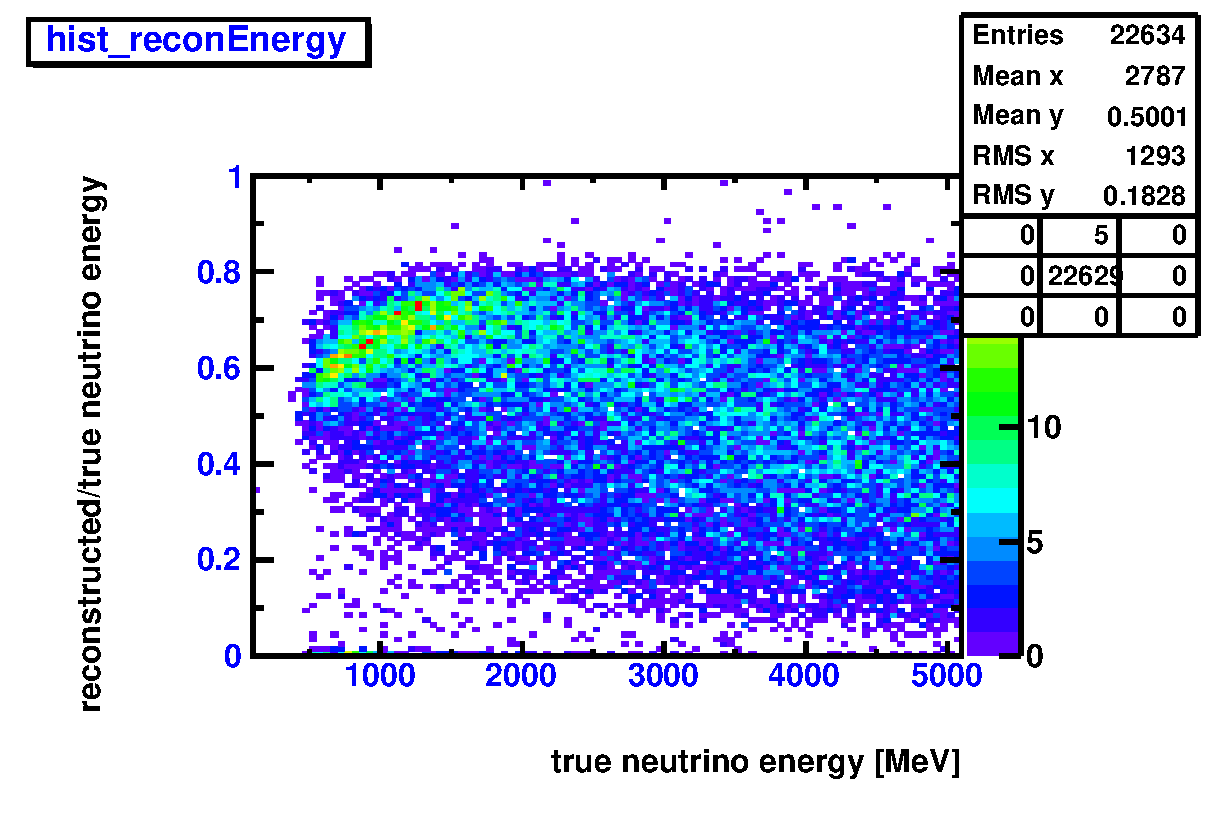
\includegraphics[width=1.0\textwidth]{analyzed_mtq_flatSpectrum_numu_H1_outerBufferFillAll_reconVSTrueEnergy_onlyCC_maxR600cm.eps}
		\column{0.3\textwidth}
		\ce{\nu_{\mu} + ^{12}C -> \mu^{-} + ?}
		\includegraphics[width=1.0\textwidth]{analyzed_mtq_flatSpectrum_numu_C12_outerBufferFillAll_reconVSTrueEnergy_onlyCC_maxR600cm.eps}
	\end{columns}
\end{frame}

\begin{frame}
	\frametitle{Energy calibration using cosmic ray $\mu$}
	\framesubtitle{Can we find more accurate $\mu$ speed when prepulse is filtered
	out?}
	\begin{center}
	\includegraphics[width=0.5\textwidth]{prepulse.png}
	\end{center}
	Algorithm:
	\begin{enumerate}
		\item threshold $\equiv 0.3 \times (\text{charge of largest pulse} Q_{2})$
		\item choose first pulse above threshold
		\item let $T = t_{2}$
		\item let $Q = Q_{1} + Q_{2} + Q_{3}$
	\end{enumerate}
	
\end{frame}

\begin{frame}
	\frametitle{Energy calibration using cosmic ray $\mu$}
	\framesubtitle{Plot PMT hit time vs angle wrt middle point of muon track}
	\begin{center}
		\includegraphics[height=0.5\textheight]{pmt_angle_wrt_muon.png}
	\end{center}
	Conditions:
	\begin{itemize}
		\item runs \numrange{5000}{5009}
		\item impact parameter $< \SI{50}{cm}$
		\item muon fitter badness $< 20$
	\end{itemize}
\end{frame}

\begin{frame}
	\frametitle{PMT hit time vs angle wrt $\mu$ center point}
	\framesubtitle{run \numrange{5000}{5009}, 204 events}
	\begin{columns}[t]
		\column{0.5\textwidth}
		Using first hits
		\includegraphics[width=1.0\textwidth]{analyzed_rtq_atm_mu_run005000_test_hitTimePositions_includeEarlyLateHits.pdf}
		\column{0.5\textwidth}
		Using first large pulse hits
		\includegraphics[width=1.0\textwidth]{analyzed_rtq_atm_mu_run005000_multiPulse_test_hitTimePositions_includeEarlyLateHits.pdf}
	\end{columns}
\end{frame}

\begin{frame}
	\frametitle{PMT hit time vs angle wrt $\mu$ center point}
	\framesubtitle{run \numrange{5000}{5009}, 204 events, 3$\sigma$ cut wrt
neighbor PMTs}
	\begin{columns}[t]
		\column{0.5\textwidth}
		Using first hits
		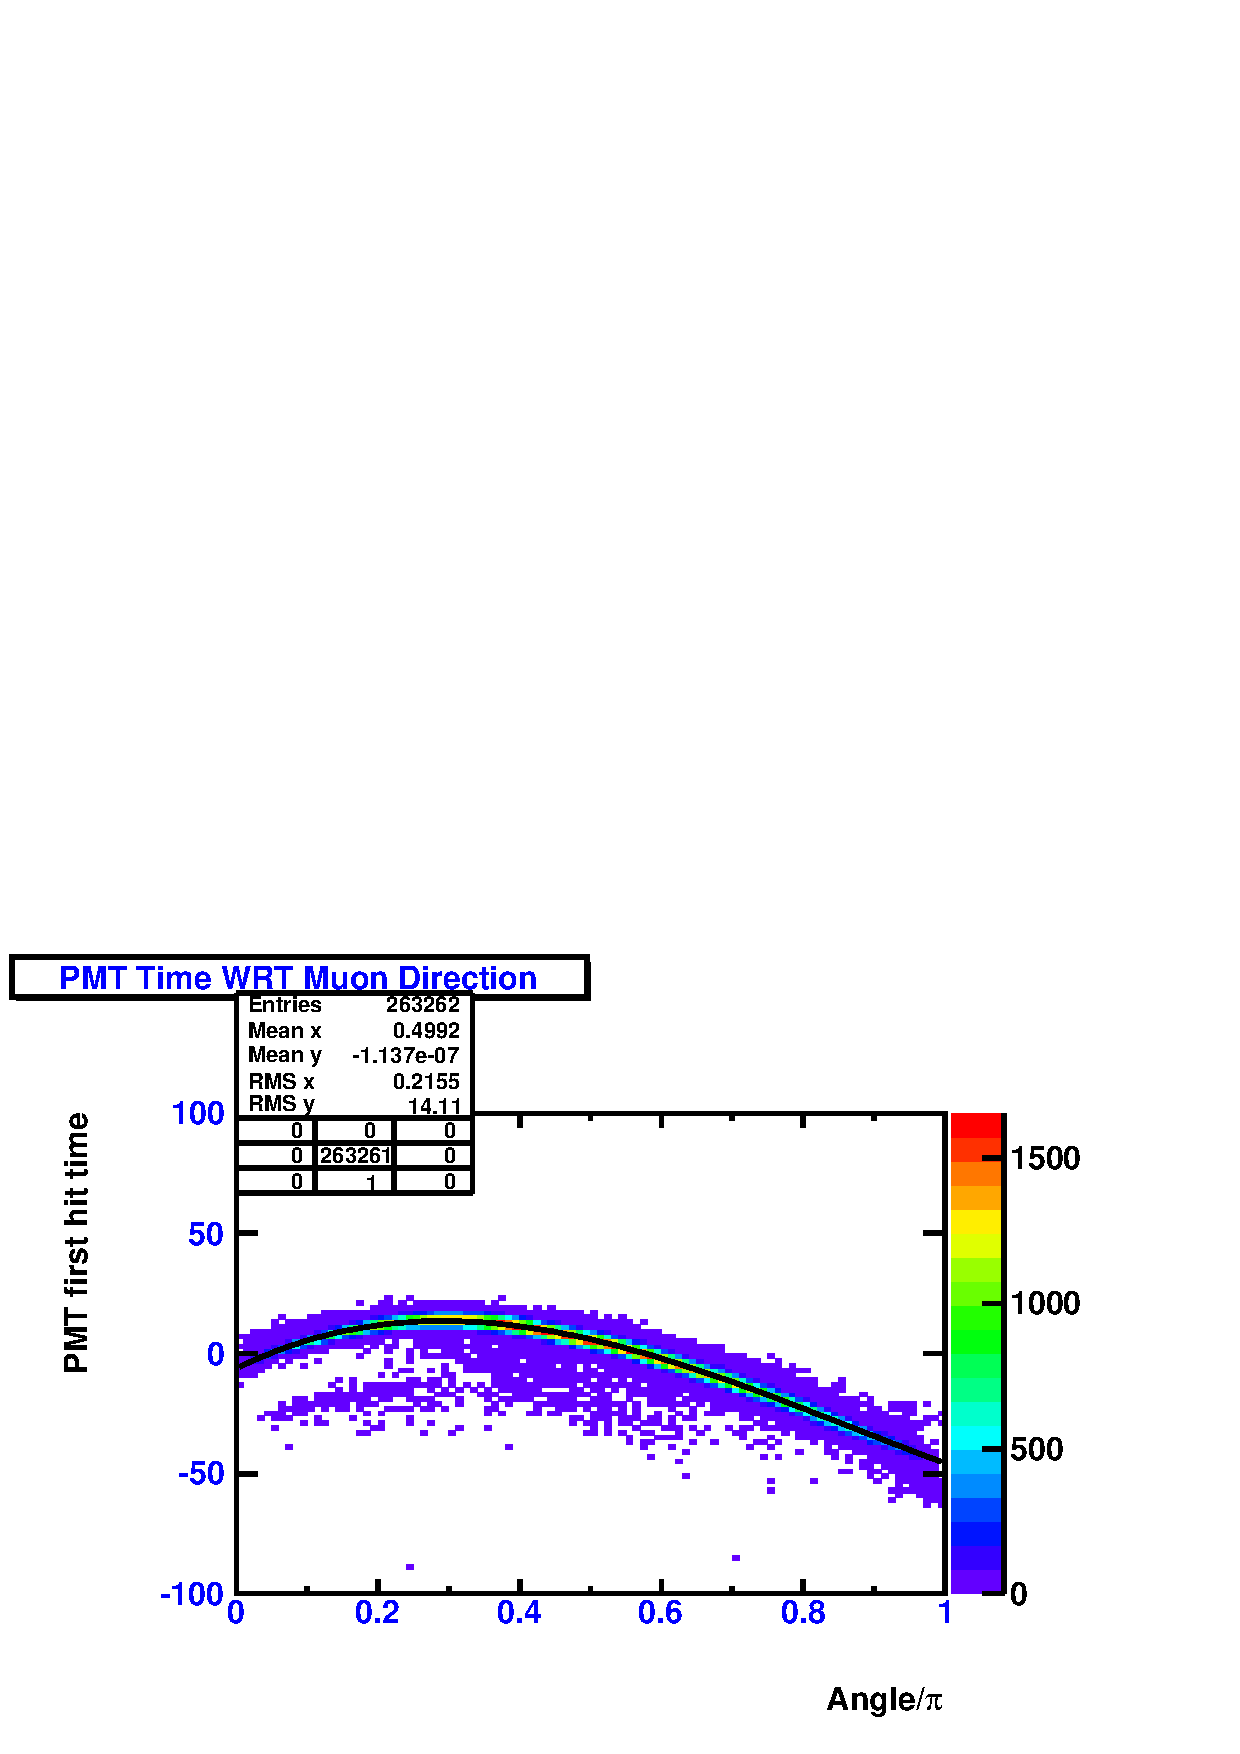
\includegraphics[width=1.0\textwidth]{analyzed_rtq_atm_mu_run005000_test_hitTimePositions.pdf}
		\column{0.5\textwidth}
		Using first large pulse hits
		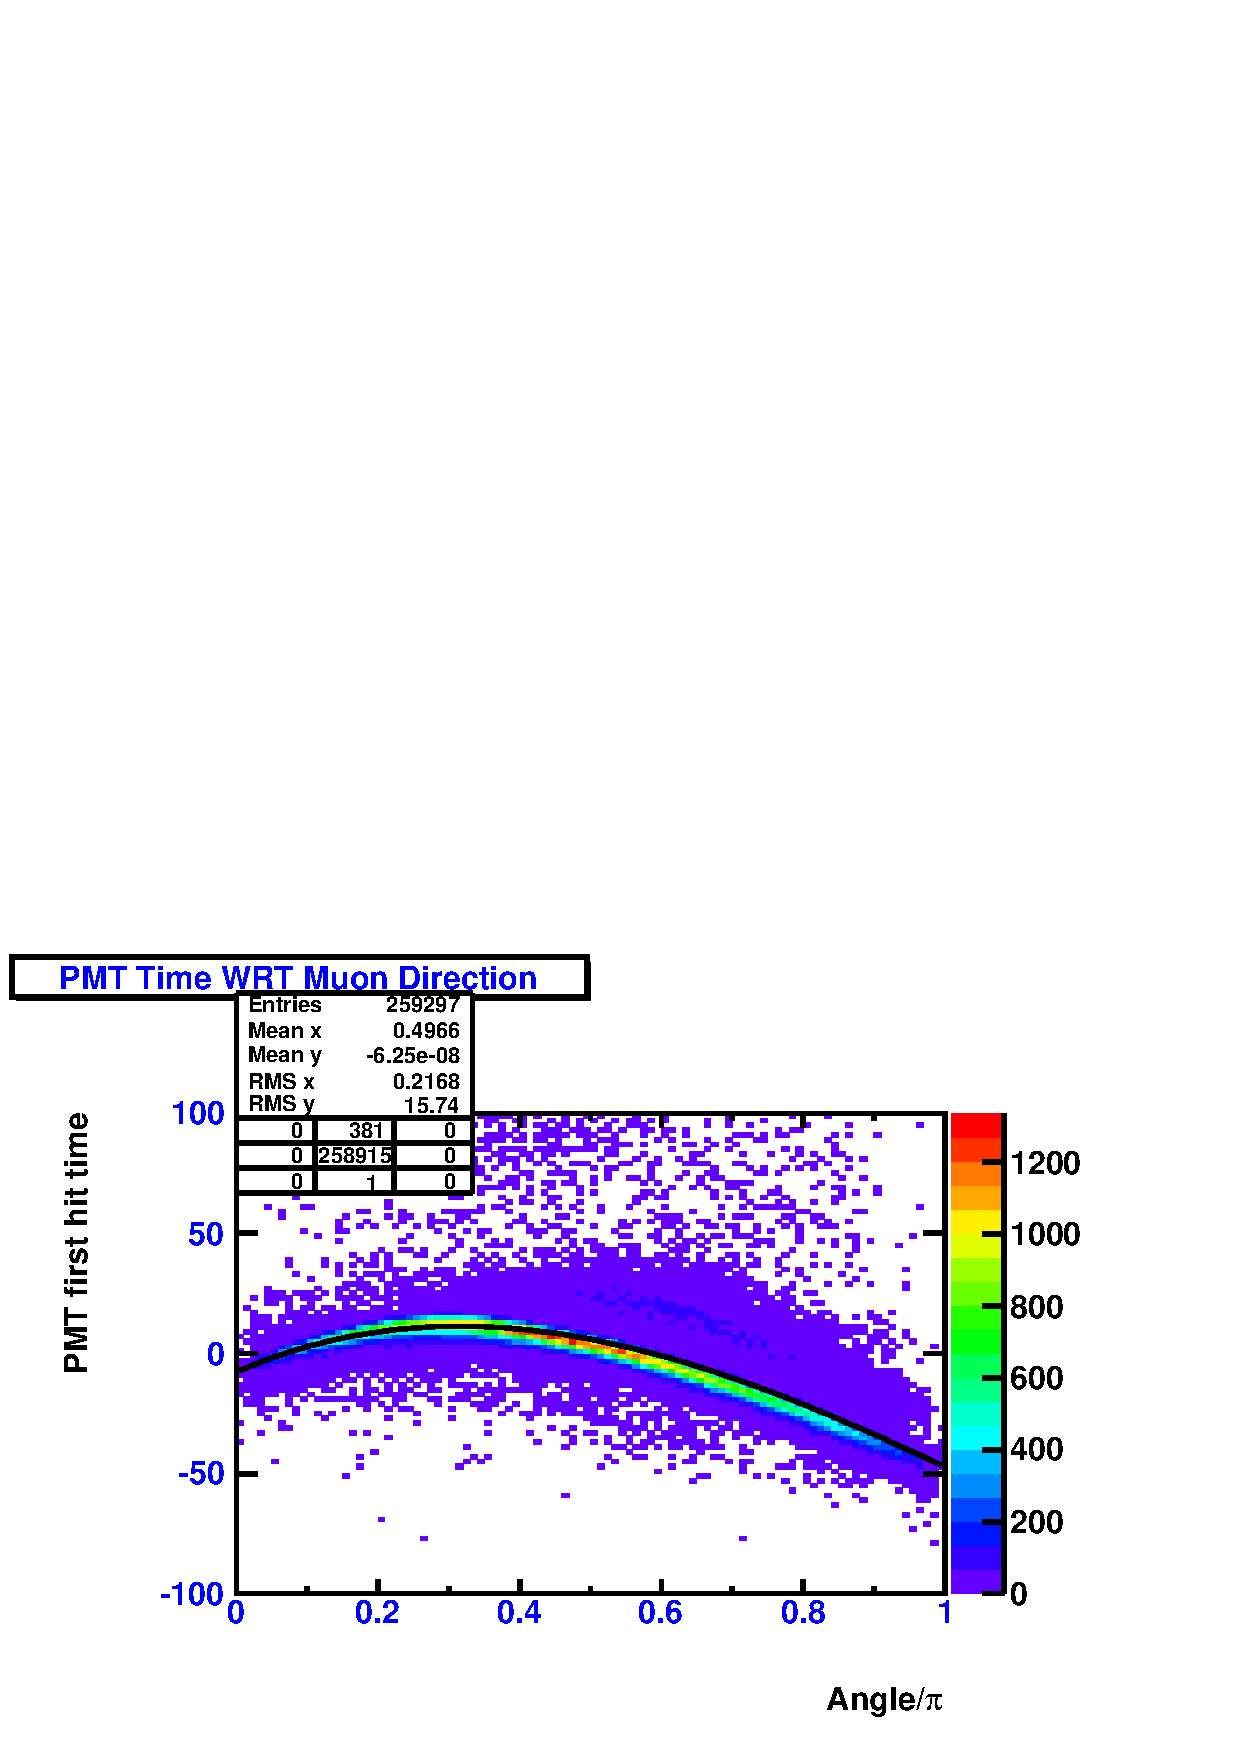
\includegraphics[width=1.0\textwidth]{analyzed_rtq_atm_mu_run005000_multiPulse_test_hitTimePositions.pdf}
	\end{columns}
\end{frame}

\begin{frame}
	\frametitle{Notes}
	
	\begin{itemize}
		\item what was defined as ``prepulse'' previously is successfully
			removed
		\item fist hit time is less precise where prepulse previously existed
			($\text{Angle}/\pi < 0.4$)
		\item many secondary pulses are included in first hits for
			$\text{Angle}/\pi > 0.5$
			(can be seen by second rainbow shape above main first hits streak)
		\item prepulses are removed around area of muon entrance?
	\end{itemize}
\end{frame}

\end{document}
